% dexcup: self-contained paper source. Compile with pdflatex (run twice for references), e.g. on Overleaf.
% All charts are drawn here with pgfplots from the numbers in the repository's results files; no image files.
\documentclass[10pt,twocolumn]{article}


\usepackage[a4paper,margin=1.9cm,columnsep=0.6cm]{geometry}
\usepackage[T1]{fontenc}
\usepackage{lmodern,microtype,amsmath,amssymb,booktabs,array,xcolor,caption,url}
\usepackage{tikz,pgfplots}
\usepackage[hidelinks]{hyperref}
\usetikzlibrary{arrows.meta,positioning,fit,calc}
\pgfplotsset{compat=1.17}
\captionsetup{font=small,labelfont=bf}
\setlength{\parskip}{0.2em}

% Colours follow the validated categorical order: identity is also given by legends and direct labels.
\definecolor{dexblue}{HTML}{2A78D6}
\definecolor{insorange}{HTML}{EB6834}
\definecolor{aquaC}{HTML}{1BAF7A}
\definecolor{ink}{HTML}{52514E}
\definecolor{gridc}{HTML}{E4E3DF}
\pgfplotsset{
  dexstyle/.style={
    width=0.96\columnwidth, height=5.0cm, axis lines=left, tick align=outside,
    tick style={ink, thin}, axis line style={ink}, ymajorgrids, grid style={gridc},
    tick label style={font=\footnotesize}, label style={font=\footnotesize},
    legend style={font=\footnotesize, draw=none, fill=none},
    legend cell align=left,
  },
}

\title{\textbf{dexcup: Call the Big Brain Only When It Matters}\\[0.3em]
\large Phase-Aware Teacher--Student Routing for Humanoid Pick-and-Place, Learned from Self-Recorded Egocentric Videos}
\author{adityavivek11}
\date{November 2026}

\begin{document}
\maketitle

\begin{abstract}
Large manipulation policies are accurate but expensive to run at control rate, yet most of a pick-and-place
requires little precision: only grasping and placing are delicate. We test whether a large \emph{teacher} policy
can be called only during those phases, with a 250-times smaller \emph{student} driving the rest and a small
\emph{router} choosing online from the robot's observation. All demonstrations originate from our own egocentric
iPhone recordings, tracked with two AprilTags, retargeted to a simulated Unitree G1 and validated by physics replay.
On 100 unseen layouts, the router succeeds on 76\% of episodes while calling the teacher on 32\% of control steps,
at an estimated 3.0 times less compute per step; the teacher alone succeeds on 86\%. A random router with the same
call rate succeeds on only 43\% (paired exact McNemar test, $p = 2.5\times10^{-7}$), showing that \emph{when} the
teacher is called matters. Repeating the pipeline on a 5-finger Inspire hand, with 20 additional recordings, gave
teacher and router success of 59\% at 2.2 times less compute, and a router advantage over random routing that was
not significant ($p = 0.23$). In this case study the identical task became substantially harder to execute with the
more complex hand. All results are in simulation.
\end{abstract}

\section{Introduction}
A humanoid policy that runs at 50\,Hz has 20\,ms per decision, shared with state estimation and control. Large
models fit this budget poorly, and running them at every step is wasteful if most steps are easy. In a
pick-and-place, reaching toward an object and carrying it tolerate centimetre-level errors, whereas the moments of
closing the fingers and letting go do not.

This suggests a simple design: use a large policy only where it matters and a small one elsewhere. Three questions
decide whether the design is useful: (1) Can a small policy handle the easy phases? (2) Can the switch be decided
online, without privileged information? (3) Does the timing of the calls matter, or would any schedule with the same
budget do equally well? The third question requires a control that many efficiency evaluations omit: a \emph{random
router} with the same teacher-call rate.

We also impose a practical constraint: demonstrations must come from cheap, self-collected data. We recorded
ourselves with a stock iPhone on the head, with no depth sensor and no motion capture.

\textbf{Contributions.}
(i) An end-to-end pipeline from phone video to a simulated humanoid policy, with physics replay as a data filter.
(ii) A phase-routed teacher--student system with a random-router control and paired significance tests.
(iii) Evidence that training the student \emph{inside} the router is what makes routing work (router success 42\% to 76\%).
(iv) A documented case study of moving the same task to a more complex 5-finger hand.
(v) A full record of what failed, including five teacher versions that did not work.

\section{Related Work}
\textbf{Action chunking.} Our teacher follows Action Chunking with Transformers (ACT)~\cite{act}, predicting
sequences of future actions and blending overlapping predictions; we omit its CVAE.
\textbf{Compounding errors.} Behaviour cloning drifts when small errors lead to unseen states. DAgger~\cite{dagger}
queries an expert on visited states; DART~\cite{dart} injects noise during demonstration collection, which needs no
queryable expert. We use DART for the teacher and DAgger for the student.
\textbf{Causal confusion.} Including history or motion in the input can make a cloned policy copy its own past
action~\cite{causalconfusion,copycat}. We observed this directly in one-step students (Section~\ref{sec:student}).
\textbf{Distillation.} Training a small model from a large one~\cite{distill} usually aims to replace it; here the
student replaces the teacher only in part of the task.
\textbf{Learning from egocentric video.} Recent systems learn robot skills from head-mounted human
data~\cite{egomimic,dexcap}, typically with dedicated sensing. We use a stock phone and fiducial markers.

\section{Task and Simulation}
\textbf{Robot.} A full Unitree G1 from MuJoCo Menagerie~\cite{mujoco,menagerie}, with its pelvis fixed at 0.793\,m;
balance is out of scope. The main result uses the 3-finger Dex3-1 hand (7 joints). Physics runs at 500\,Hz with the
implicit-fast integrator, and the policy at 50\,Hz.

\textbf{Objects.} Dimensions match the real objects: a cardboard tube (radius 4.7\,cm, height 17.8\,cm) and a
tape-roll coaster (radius 4.5\,cm, height 2\,cm, collidable, so the tube rests on it). The tube's mass, 0.15\,kg,
was assumed and not weighed.

\textbf{Control.} The action is a palm position target and a binary grip. Damped-least-squares inverse kinematics
with a null-space posture term and warm starts converts the target to seven arm joint targets, with hand orientation
fixed. Finger servos are softened ($k_p = 20$) because the stock gain launches the tube.

\textbf{Grasp check.} A grasp is confirmed when the thumb's distal link and at least one opposing finger's distal
link each press on the tube with more than 0.5\,N.

\textbf{Success.} The tube must stay within 3\,cm of the coaster centre, upright, raised onto the coaster, and not
grasped, for 1\,s (50 ticks), within 20\,s (1000 ticks). The ``released'' condition was first defined as zero finger
contact and later changed to ``not grasped'' after we had seen results from an early teacher, because the original
was stricter than both the grasp definition and the replay filter that built the training data. We disclose this
post-hoc change; it predates all results reported here.

\begin{figure*}[t]
\centering
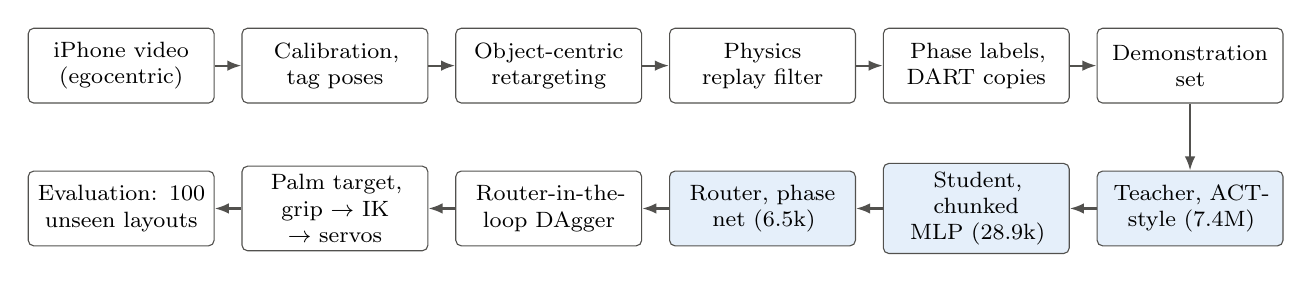
\begin{tikzpicture}[
  node distance=0.34cm and 0.34cm,
  box/.style={draw=ink, rounded corners=2pt, align=center, font=\footnotesize, minimum height=0.95cm, inner sep=3pt, text width=2.15cm},
  key/.style={box, fill=dexblue!12},
  arr/.style={-{Latex[length=1.8mm]}, ink, thick}]
\node[box] (rec) {iPhone video\\(egocentric)};
\node[box,right=of rec] (trk) {Calibration, tag poses};
\node[box,right=of trk] (ret) {Object-centric retargeting};
\node[box,right=of ret] (phy) {Physics replay filter};
\node[box,right=of phy] (lab) {Phase labels, DART copies};
\node[box,right=of lab] (dem) {Demonstration set};
\draw[arr] (rec)--(trk); \draw[arr] (trk)--(ret); \draw[arr] (ret)--(phy); \draw[arr] (phy)--(lab); \draw[arr] (lab)--(dem);
\node[key,below=0.85cm of dem] (tea) {Teacher, ACT-style (7.4M)};
\node[key,left=of tea] (stu) {Student, chunked MLP (28.9k)};
\node[key,left=of stu] (rou) {Router, phase net (6.5k)};
\node[box,left=of rou] (rd) {Router-in-the-loop DAgger};
\node[box,left=of rd] (ctl) {Palm target, grip $\to$ IK $\to$ servos};
\node[box,left=of ctl] (ev) {Evaluation: 100 unseen layouts};
\draw[arr] (dem)--(tea); \draw[arr] (tea)--(stu); \draw[arr] (stu)--(rou); \draw[arr] (rou)--(rd); \draw[arr] (rd)--(ctl); \draw[arr] (ctl)--(ev);
\end{tikzpicture}
\caption{Pipeline from recordings to evaluation. Every training episode originates from one of our recordings; no
scripted or generic demonstrations are mixed in.}
\label{fig:pipeline}
\end{figure*}

\section{From Phone Video to Demonstrations}
Figure~\ref{fig:pipeline} summarises the pipeline. Each demonstration supplies the tube's start, the coaster's
position, the carry path and the timing. The robot supplies what a human video cannot: its own measured grasp and
scripted approach and retreat paths, retimed to the human's durations.

\textbf{Recording.} A head-mounted iPhone with its stock camera: 1080p, 30\,fps, 0.5$\times$ lens, HDR and enhanced
stabilisation off, exposure and focus locked. Each clip holds one demonstration, with the tube and coaster moved
between clips. Of 67 clips, 62 passed the quality gate. Portrait orientation (mean wrist-tag visibility 87\%) beat
landscape (72\%), and moving slower raised visibility from 79\% to 95\% and cut the median longest tracking gap from
0.9\,s to 0.2\,s.

\textbf{Calibration.} A checkerboard video gives the intrinsics~\cite{zhang}. Fitting $f_x$, $f_y$, $c_x$ and $c_y$
freely gave $f_x{=}884$, $f_y{=}889$ pixels (about 95$^\circ$ horizontal field of view) and RMS error 0.43\,px.
Forcing $f_x{=}f_y$ raised RMS to 0.68\,px and shifted $f_x$ by about 9\%, likely because of anisotropic printer
scaling. Printed sizes were scaled by 0.96 to match the measured print.

\textbf{Tracking.} Two tag36h11 AprilTags~\cite{apriltag,apriltag2} are used: ID~1 beside the coaster (67.2\,mm), which
defines the world frame, and ID~0 on the back of the right wrist (33.6\,mm). We replaced OpenCV's ArUco detector with
pupil-apriltags because it missed the slightly curved wrist tag, and solve each pose with planar PnP~\cite{ippe},
rejecting detections by reprojection error. When the hand hides the coaster tag (1.6--2.5\,s during placing), a
checkerboard fixed to the table acts as a second static anchor. On synthetic sequences the tracker's error was median
1.5\,mm, 95th percentile 3.5\,mm and 0.4$^\circ$.

\textbf{Coaster location.} The roll was moved between clips, so it is located per clip by rectifying its top-rim plane
into a metric top view and fitting a 45\,mm circle. Fits had radius 43--47\,mm and spread of at most 1.5\,mm; a fixed
assumed position would have been wrong by up to 4\,cm.

\textbf{Object-centric retargeting.} Copying wrist poses directly fails because the two hands differ, so the robot
uses its own grasp, swept empirically: palm offset from the tube centre $(-0.13, -0.0625, 0)$\,m, within a working
window only about 1\,cm wide in $x$. There is no tube tag, so its path is reconstructed by running the carry backwards
from the place moment, assuming the tube is rigid in the hand. Human positions map to the robot as
\begin{equation}
\mathbf{x}_r = S\,\mathbf{R}\,(\mathbf{x}_h - \mathbf{h}_h) + \mathbf{h}_r + \boldsymbol{\Delta},
\end{equation}
where $\mathbf{R}$ aligns the camera's horizontal facing direction with the robot's $+x$, $\mathbf{h}$ is the head
position, $S=0.3$ is a horizontal scale, and $\boldsymbol{\Delta}$ is one shift shared by all clips, chosen to centre
them on the robot's \emph{measured} workspace (Figure~\ref{fig:reach}). Approach and retreat are one continuous eased
motion each, since easing to full stops created fixed points where a state-based policy hovered indefinitely. Pauses
of 0.6\,s and 0.5\,s let the fingers close and open. Human finger motion is not retargeted.

\textbf{Physics validation.} Each plan is replayed in MuJoCo through the same control loop the policies use; only
physical successes are kept. Table~\ref{tab:data} shows the outcomes. Episodes last 9.0--19.4\,s (median 14.1\,s).

\textbf{Phase labels.} Approach, grasp, transport, place and retreat are assigned by physics-only rules using palm
pose, tube lift, distance to the coaster and finger contact. They agree with the planned phases on 84\% of ticks, and
grasp plus place cover 25\% of ticks.

\begin{table}[t]
\centering\small
\caption{Data at each stage for both hands.}
\label{tab:data}
\begin{tabular}{@{}lrr@{}}
\toprule
 & Dex3-1 & Inspire \\
\midrule
Clips tracked & 62 & 82 \\
Fail: tube-start height check & 7 & 7 \\
Fail: outside workspace & 7 & 6 \\
Fail: placed off target or toppled & 5 & 7 \\
Fail: dropped in carry & 2 & 1 \\
\textbf{Successful replays} & \textbf{41} & \textbf{61} \\
Training / held-out clips & 32 / 9 & 48 / 13 \\
DART noise $\sigma$ & 1.0\,cm & 0.5\,cm \\
DART replays kept / run & 75/164 & 119/192 \\
DART replays of training clips & 56 & 119 \\
\textbf{Training episodes} & \textbf{88} & \textbf{167} \\
\bottomrule
\end{tabular}
\end{table}

\textbf{DART.} For robustness, each clip is replayed four times with Ornstein--Uhlenbeck noise on the \emph{executed}
target and the clean target recorded as the label:
\begin{equation}
\mathbf{n}_{t+1} = (1-a)\,\mathbf{n}_t + \sigma\sqrt{2a}\,\boldsymbol{\epsilon}_t,\quad a=\frac{\Delta t}{\tau},
\end{equation}
with $\Delta t = 0.02$\,s, $\tau=0.5$\,s, and no noise while the fingers close or open. Only noisy replays that still
succeed are kept, and only for training clips, so no held-out layout leaks into training. Held-out clips were frozen
before training.

\section{Policies}
\textbf{Observation.} 38 numbers from the simulator state: palm position (3), tube position (3), tube axis (3),
coaster position (2), finger joints (7), arm joints (7), tube-minus-palm and coaster-minus-tube vectors (6), and arm
joint velocities (7). Student and router use the first 31. Policies therefore assume known object state; there are no
images and no language input.

\textbf{Teacher (7.4M parameters).} A transformer ($d{=}256$, 4 layers, 8 heads) over tokens for grouped observation
features, with $H{=}16$ learned queries predicting a chunk of palm targets relative to the current palm, plus grip
logits. The loss is mean squared position error in centimetres plus binary cross-entropy on the grip. At run time,
overlapping chunks are converted to absolute targets and blended with weights $w_k \propto \exp(-0.1\,k)$, where $k$
is the chunk's age in ticks. Training ran for 80 epochs on a Kaggle T4 GPU (about 30 minutes).

\textbf{Student (28.9k parameters).}\label{sec:student} An MLP with two hidden layers of 128 units and the same chunked
output and blending, without velocity inputs. It is trained by behaviour cloning on demonstrations and DART copies, then
by DAgger with mixing $\beta_k = 0.5^k$ (4 rounds of 24 rollouts), then by router-in-the-loop DAgger: rollouts are
driven by the real router, and a separate copy of the teacher labels every tick the student drives (4 rounds of 36
rollouts, half on training layouts and half on fresh layouts drawn with different seeds from the test set). The best
round is selected on 40 further layouts (seed 2000): 78\%, 85\% and 82\% for the three saved rounds, selecting the second.
A laptop shutdown interrupted the first router-DAgger run; the reported rounds continue from the student it had saved, with
its collected data lost.

Earlier student designs failed. A one-step MLP \emph{with} velocities learned to continue its current motion, a
feedback loop consistent with the copycat problem~\cite{copycat}: its targets ran metres away within about 10 ticks,
and the runaway rollouts inflated the normalisation statistics about 50-fold (now fixed from the demonstrations). A
one-step MLP \emph{without} velocities did not explode but drifted, with 0 of 6 grasps. The chunked version grasped on
4 of 6 layouts from behaviour cloning alone.

\textbf{Router (6.5k parameters).} A two-hidden-layer MLP (64 units) classifying the five phases from the observation
(93\% accuracy on held-out clips). The teacher is called when the predicted phase is grasp or place. Ground-truth
labels and contacts are never read at test time. Each model's chunk buffer is reset when its segment begins, so stale
predictions are not blended in.

\section{Evaluation Protocol}
\textbf{Layouts.} 100 layouts (seed 0), sampled uniformly over the training bounding box, with tube and coaster at
least 10\,cm apart and inside the measured workspace, unseen during training and selection.

\textbf{Conditions.} Teacher only, student only, router, and random router. The random router is a two-state Markov
chain with switching probabilities
\begin{equation}
P(\text{to teacher}) = \frac{p}{L(1-p)},\quad P(\text{to student}) = \frac{1}{L},
\end{equation}
which matches the router's teacher-call fraction $p$ and mean teacher-segment length $L$, so the control differs from
the router only in \emph{when} it calls the teacher, not how much or how long.

\textbf{Statistics.} Success rates carry 95\% Wilson intervals. Conditions are compared on the same layouts with the
exact two-sided McNemar test~\cite{mcnemar}: under no difference, each discordant layout is a fair coin flip.

\textbf{Latency.} Each model is timed for 3000 forward passes in one process on one thread, on an Intel i5-12450H
laptop CPU. Compute per step is an estimate, not an end-to-end measurement:
\begin{equation}
c = f\,t_T + (1-f)\,t_S + t_P,
\end{equation}
where $f$ is the teacher-call fraction and $t_T$, $t_S$, $t_P$ are teacher, student and phase-net times ($t_P$ applies
to the router only). Absolute times varied with the machine's power state (the teacher measured 8--23\,ms across
sessions), while the ratio stayed near 3; only timings from one session are compared.

\section{Results}
\begin{table}[t]
\centering\small
\caption{Main result: G1 with Dex3-1 on 100 unseen layouts. Success with 95\% Wilson interval; $c$ estimated by Eq.~(4).}
\label{tab:main}
\setlength{\tabcolsep}{3pt}
\begin{tabular}{@{}lcccc@{}}
\toprule
Policy & Success (\%) & Teacher & $c$ (ms) & Calls per\\
 & & calls & & success\\
\midrule
Teacher only & 86 [78, 92] & 100\% & 7.97 & 558\\
\textbf{Router} & \textbf{76} [67, 83] & \textbf{32\%} & \textbf{2.64} & \textbf{226}\\
Random router & 43 [34, 53] & 31\% & 2.48 & 545\\
Student only & 16 [10, 24] & 0\% & 0.05 & --\\
\bottomrule
\end{tabular}
\end{table}

\begin{figure}[t]
\centering
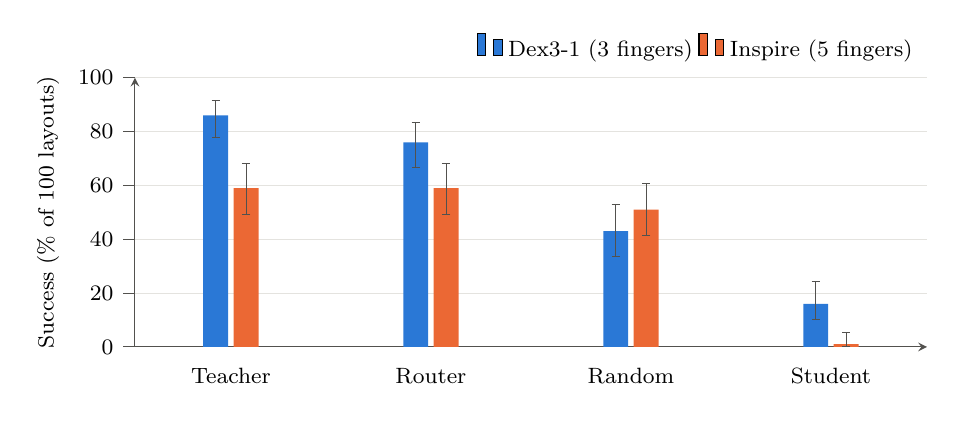
\begin{tikzpicture}
\begin{axis}[dexstyle, ybar, bar width=9pt, enlarge x limits=0.16, ymin=0, ymax=100, ylabel={Success (\% of 100 layouts)},
  symbolic x coords={Teacher,Router,Random,Student}, xtick=data, xtick style={draw=none},
  legend style={at={(1,1.02)},anchor=south east,legend columns=2},
  error bars/error bar style={ink}, error bars/error mark options={rotate=90,mark size=1.5pt,ink}]
\addplot[fill=dexblue,draw=none,error bars/.cd,y dir=both,y explicit] coordinates {
 (Teacher,86) += (0,5.5) -= (0,8.1) (Router,76) += (0,7.3) -= (0,9.2) (Random,43) += (0,9.8) -= (0,9.3) (Student,16) += (0,8.4) -= (0,5.9)};
\addlegendentry{Dex3-1 (3 fingers)}
\addplot[fill=insorange,draw=none,error bars/.cd,y dir=both,y explicit] coordinates {
 (Teacher,59) += (0,9.1) -= (0,9.8) (Router,59) += (0,9.1) -= (0,9.8) (Random,51) += (0,9.6) -= (0,9.7) (Student,1) += (0,4.4) -= (0,0.8)};
\addlegendentry{Inspire (5 fingers)}
\end{axis}
\end{tikzpicture}
\caption{Closed-loop success on 100 test layouts per hand. Each hand uses layouts from its own workspace, so the two
are not tested on identical positions. Whiskers are 95\% Wilson intervals.}
\label{fig:success}
\end{figure}

Table~\ref{tab:main} and Figure~\ref{fig:success} give the main result. The router succeeds on 76\% of layouts while
calling the teacher on 32\% of control steps, 3.0 times less estimated compute per step than the teacher alone.
It costs 10 percentage points of success: on the same layouts, the teacher alone is better on 12 and the router on 2
($p = 0.013$).

\textbf{Timing matters.} The random router uses the same teacher budget and reaches only 43\%. The router is better on 38
layouts and the random router on 5 ($p = 2.5\times10^{-7}$). Teacher calls per successful episode are 226 vs 545.
Figure~\ref{fig:tradeoff} places all conditions on the success--compute plane, and Figure~\ref{fig:latency} gives
per-model timing.

\begin{figure}[t]
\centering
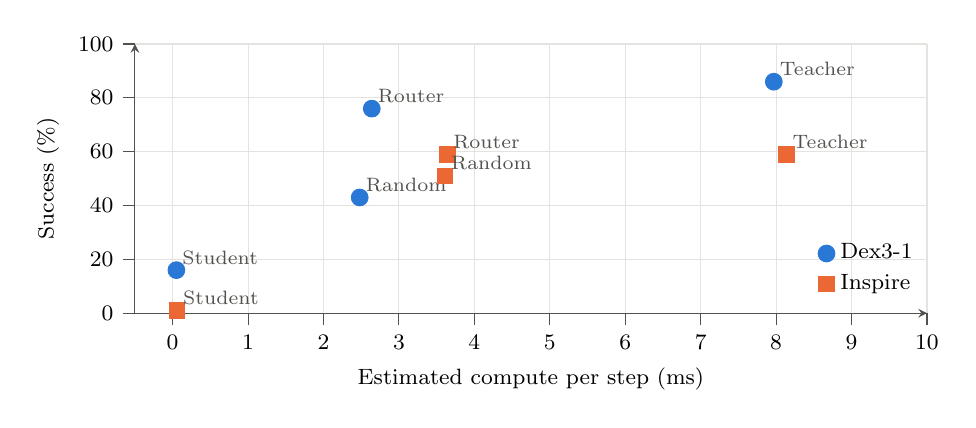
\begin{tikzpicture}
\begin{axis}[dexstyle, xlabel={Estimated compute per step (ms)}, ylabel={Success (\%)}, xmin=-0.5, xmax=10, ymin=0, ymax=100,
  xmajorgrids, legend style={at={(1,0.03)},anchor=south east},
  nodes near coords, point meta=explicit symbolic, every node near coord/.style={font=\scriptsize,text=ink,anchor=south west,inner sep=2pt}]
\addplot[only marks,mark=*,mark size=3pt,dexblue] coordinates {(7.97,86)[Teacher] (2.64,76)[Router] (2.48,43)[Random] (0.05,16)[Student]};
\addlegendentry{Dex3-1}
\addplot[only marks,mark=square*,mark size=2.8pt,insorange] coordinates {(8.14,59)[Teacher] (3.64,59)[Router] (3.61,51)[Random] (0.06,1)[Student]};
\addlegendentry{Inspire}
\end{axis}
\end{tikzpicture}
\caption{Success against estimated compute. The upper left is best. The Dex3-1 router sits well above the random
router at about the same compute.}
\label{fig:tradeoff}
\end{figure}

\begin{figure}[t]
\centering
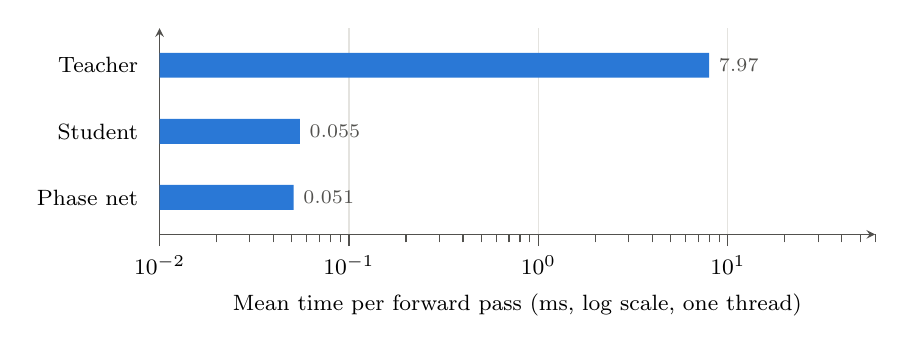
\begin{tikzpicture}
\begin{axis}[dexstyle, width=0.88\columnwidth, height=4.2cm, xbar, bar width=9pt, xmode=log, log origin=infty, xmin=0.01, xmax=60, ymajorgrids=false, xmajorgrids,
  xlabel={Mean time per forward pass (ms, log scale, one thread)}, symbolic y coords={Phase net,Student,Teacher}, ytick=data, ytick style={draw=none},
  enlarge y limits=0.28, point meta=rawx, nodes near coords, nodes near coords align={horizontal}, nodes near coords style={font=\scriptsize,text=ink,/pgf/number format/fixed,/pgf/number format/precision=3}]
\addplot[fill=dexblue,draw=none] coordinates {(0.051,Phase net) (0.055,Student) (7.97,Teacher)};
\end{axis}
\end{tikzpicture}
\caption{Per-model latency for the Dex3-1 models. 95th percentiles: teacher 10.40\,ms, student 0.065\,ms, phase net 0.077\,ms.}
\label{fig:latency}
\end{figure}

\begin{figure}[t]
\centering
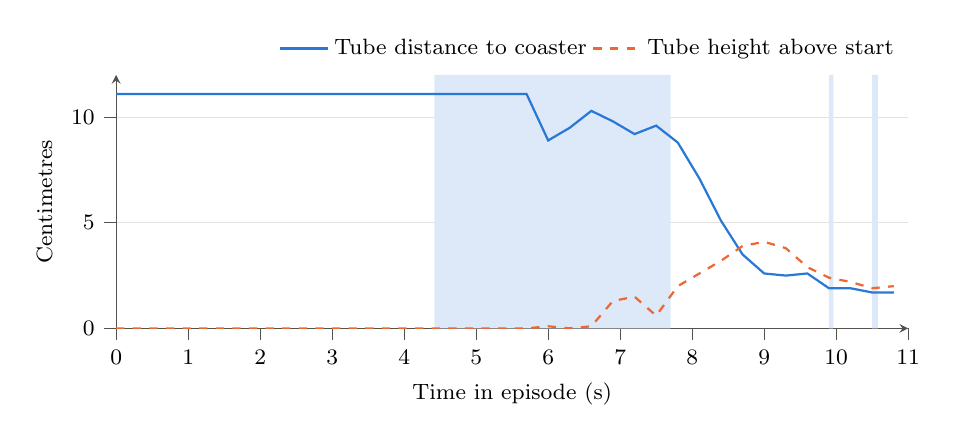
\begin{tikzpicture}
\begin{axis}[dexstyle, height=4.8cm, xlabel={Time in episode (s)}, ylabel={Centimetres}, xmin=0, xmax=11, ymin=0, ymax=12,
  legend style={at={(1,1.02)},anchor=south east,legend columns=2}]
\addplot[fill=dexblue!16,draw=none,forget plot] coordinates {(4.42,0) (4.42,12) (7.70,12) (7.70,0)} \closedcycle;
\addplot[fill=dexblue!16,draw=none,forget plot] coordinates {(9.90,0) (9.90,12) (9.96,12) (9.96,0)} \closedcycle;
\addplot[fill=dexblue!16,draw=none,forget plot] coordinates {(10.50,0) (10.50,12) (10.58,12) (10.58,0)} \closedcycle;
\addplot[thick,dexblue,no marks] coordinates {(0,11.1) (0.3,11.1) (0.6,11.1) (0.9,11.1) (1.2,11.1) (1.5,11.1) (1.8,11.1) (2.1,11.1) (2.4,11.1) (2.7,11.1) (3.0,11.1) (3.3,11.1) (3.6,11.1) (3.9,11.1) (4.2,11.1) (4.5,11.1) (4.8,11.1) (5.1,11.1) (5.4,11.1) (5.7,11.1) (6.0,8.9) (6.3,9.5) (6.6,10.3) (6.9,9.8) (7.2,9.2) (7.5,9.6) (7.8,8.8) (8.1,7.1) (8.4,5.1) (8.7,3.5) (9.0,2.6) (9.3,2.5) (9.6,2.6) (9.9,1.9) (10.2,1.9) (10.5,1.7) (10.8,1.7)};
\addlegendentry{Tube distance to coaster}
\addplot[thick,insorange,dashed,no marks] coordinates {(0,0) (0.3,0) (0.6,0) (0.9,0) (1.2,0) (1.5,0) (1.8,0) (2.1,0) (2.4,0) (2.7,0) (3.0,0) (3.3,0) (3.6,0) (3.9,0) (4.2,0) (4.5,0) (4.8,0) (5.1,0) (5.4,0) (5.7,0) (6.0,0.1) (6.3,0) (6.6,0.1) (6.9,1.3) (7.2,1.5) (7.5,0.6) (7.8,2.0) (8.1,2.6) (8.4,3.2) (8.7,3.9) (9.0,4.1) (9.3,3.8) (9.6,2.9) (9.9,2.4) (10.2,2.2) (10.5,1.9) (10.8,2.0)};
\addlegendentry{Tube height above start}
\end{axis}
\end{tikzpicture}
\caption{One real router episode (Dex3-1, test layout 0, success, 164 of 542 ticks on the teacher). Shaded bands mark
teacher calls. In this episode the teacher covers the grasp and lift in long segments and is called only briefly
during the place phase.}
\label{fig:trace}
\end{figure}

\textbf{An example episode.} Figure~\ref{fig:trace} traces one successful episode. The student approaches; the router
hands over before the fingers close; the teacher grasps and lifts; the student carries and lowers the tube; the tube
settles on the 2\,cm roll. Most teacher ticks in this episode fall in the grasp phase, consistent with phase labels
in which grasp covers 20\% of ticks and place 5\%.

\textbf{Why the student alone fails.} The student reaches 16\% alone, yet the router reaches 76\%: the two are
complementary: the student was trained on the states it meets inside the router, where the teacher handles the delicate
phases, so its score alone does not predict its value there. Runs ending at the 20\,s limit rather than by a fall (timeouts) were 9, 19, 49
and 80 of 100 for teacher, router, random router and student.

\textbf{What made routing work.} Figure~\ref{fig:dagger} compares routers before and after router-in-the-loop DAgger. Before, the
student reached 2\% alone and the router 42\% vs random 37\% (23 vs 18 discordant, $p = 0.53$): with a student unable to
handle its phases, any 15\% mix of teacher calls landed near 40\%. Training the student inside the router raised
the router to 76\% and made timing significant. The teacher-call fraction rose from 15\% to 32\% because more
episodes now reach the phases that call the teacher (118 to 172 calls per episode).

\begin{figure}[t]
\centering
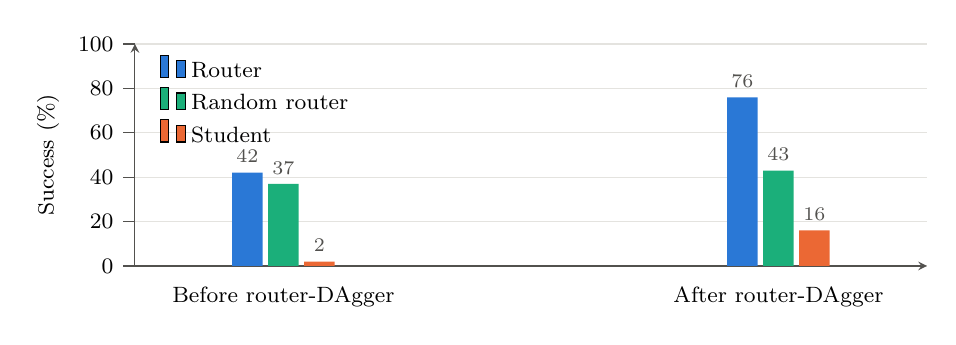
\begin{tikzpicture}
\begin{axis}[dexstyle, height=4.4cm, ybar, bar width=11pt, enlarge x limits=0.3, ymin=0, ymax=100, ylabel={Success (\%)},
  symbolic x coords={Before,After}, xtick=data, xticklabels={Before router-DAgger,After router-DAgger}, xtick style={draw=none},
  nodes near coords, nodes near coords style={font=\scriptsize,text=ink}, legend style={at={(0.02,0.98)},anchor=north west}]
\addplot[fill=dexblue,draw=none] coordinates {(Before,42) (After,76)}; \addlegendentry{Router}
\addplot[fill=aquaC,draw=none] coordinates {(Before,37) (After,43)}; \addlegendentry{Random router}
\addplot[fill=insorange,draw=none] coordinates {(Before,2) (After,16)}; \addlegendentry{Student}
\end{axis}
\end{tikzpicture}
\caption{Effect of router-in-the-loop DAgger (Dex3-1, same 100 layouts). The teacher, at 86\%, is unchanged.}
\label{fig:dagger}
\end{figure}

\textbf{Scope of the experiment.} Pick-and-place may look like a very simple experiment. That choice was due to time
constraints: this entire project, from recording to evaluation, was built in days. The same method can be applied to
many other robotic tasks, because it needs only a task with identifiable delicate phases, demonstrations and a
learnable phase signal, and none of its components is specific to tubes or coasters. Such tasks include insertion,
tool use and assembly. We have not yet tested other tasks, so how much saving they would allow remains an open question.

\section{Teacher Development}
Table~\ref{tab:versions} and Figure~\ref{fig:versions} record the path to the working teacher. Validation loss was a
poor guide: v1 reached 0.19\,cm position RMSE and still succeeded on 0 of 9 layouts, so every version was judged in closed loop.
With 9 episodes the standard error is about $\pm$14 points, so small differences between versions are not meaningful.

\begin{table}[t]
\centering\footnotesize
\caption{Teacher versions (Dex3-1, 9 held-out layouts).}
\label{tab:versions}
\setlength{\tabcolsep}{3pt}
\begin{tabular}{@{}l>{\raggedright\arraybackslash}p{3.0cm}c>{\raggedright\arraybackslash}p{3.0cm}@{}}
\toprule
Ver. & Change & Success & Finding\\
\midrule
v1 & Baseline & 0/9 & Chunk-target bug; hand crawls; corner-cutting\\
v2 & Bug fix, DART & 2/9 & Stalls at waypoints that eased to full stops\\
v3 & Continuous motions & 2/9 & Never closes or releases: labels favour ``open''\\
v4 & Grip label 0.16\,s early & 1/9 & Stops short; reverted\\
v5 & Object-relative actions & 0/9 & Parks at clearance corner\\
ov & Object-relative + velocity & 1/9 & Val.\ loss 4$\times$ worse; dropped\\
\textbf{pv} & \textbf{Palm-relative + velocity} & \textbf{7/9} & \textbf{86\% on 100 test layouts}\\
\bottomrule
\end{tabular}
\end{table}

\begin{figure}[t]
\centering
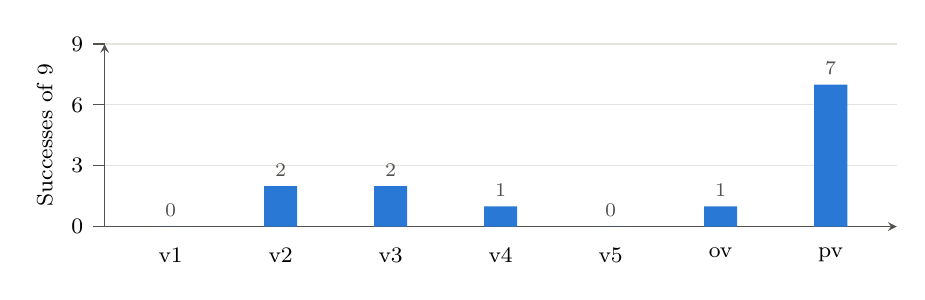
\begin{tikzpicture}
\begin{axis}[dexstyle, height=3.9cm, ybar, bar width=12pt, enlarge x limits=0.1, ymin=0, ymax=9, ytick={0,3,6,9}, ylabel={Successes of 9},
  symbolic x coords={v1,v2,v3,v4,v5,ov,pv}, xtick=data, xtick style={draw=none}, nodes near coords, nodes near coords style={font=\scriptsize,text=ink}]
\addplot[fill=dexblue,draw=none] coordinates {(v1,0) (v2,2) (v3,2) (v4,1) (v5,0) (ov,1) (pv,7)};
\end{axis}
\end{tikzpicture}
\caption{Held-out success by teacher version. Each version's failure pointed to the same gap: a state-only policy
cannot tell ``arriving at a point'' from ``leaving it''.}
\label{fig:versions}
\end{figure}

The common thread was missing motion information. In the demonstrations the hand decelerates near waypoints, and the
actions there shrink to about zero, creating apparent fixed points for a policy that sees only position. Adding seven arm
joint velocities resolved this. The same inputs that fixed the chunked teacher destabilised the one-step student, a
contrast we attribute to chunking and ensembling smoothing the feedback loop.

\section{Case Study: A 5-Finger Hand}
We repeated the pipeline with Unitree's Inspire RH56DFQ model~\cite{unitreeros} on the same G1 body (12 joints, 6 motors,
coupled joints as equality constraints), adding 20 new recordings of 5-finger grasps. All 20 succeeded in replay.
Table~\ref{tab:inspire} gives the results.

\begin{table}[t]
\centering\small
\caption{Inspire hand on 100 layouts from its own workspace.}
\label{tab:inspire}
\setlength{\tabcolsep}{3pt}
\begin{tabular}{@{}lcccc@{}}
\toprule
Policy & Success (\%) & Teacher & $c$ (ms) & Calls per\\
 & & calls & & success\\
\midrule
Teacher only & 59 [49, 68] & 100\% & 8.14 & 1253\\
Router & 59 [49, 68] & 44\% & 3.64 & 561\\
Random router & 51 [41, 61] & 44\% & 3.61 & 703\\
Student only & 1 [0, 5] & 0\% & 0.06 & --\\
\bottomrule
\end{tabular}
\end{table}

The router matched the teacher (5 vs 5 discordant layouts, $p = 1$) at 2.2 times less compute, but the advantage over the
random router was not significant (21 vs 13, $p = 0.23$), and the teacher itself was much weaker despite about twice
the training episodes. Moving to this hand required:

\begin{itemize}\setlength{\itemsep}{1pt}
\item \textbf{A new grasp.} The Dex3-style side grasp completed no pick-and-place in two sweeps of 144
configurations each, because the thumb's base protrudes from the palm where the tube would rest. The working grasp pre-shapes
the thumb across the palm and descends over the tube. The working window was again about 1\,cm wide.
\item \textbf{Physics corrections.} The URDF has no joint damping or armature and its finger links weigh about 4\,g: the
index closed in 54\,ms, tunnelled into the tube and threw it from the table. We added damping and armature for a closing
time of about 0.5\,s, and torsional friction (condim 4) to represent soft finger pads.
\item \textbf{De-weighting two fingers.} See Table~\ref{tab:hold}: with all fingers at full squeeze, thumb and fingers
formed a couple that tipped the tube about 30$^\circ$ within 4\,s in the air.
\item \textbf{Lower noise.} All 192 DART replays failed at $\sigma = 1$\,cm; at 0.5\,cm, 119 succeeded.
\item \textbf{New label rules.} Grasp-start and place-end rules assumed a sideways approach and were replaced for this
hand (agreement with planned phases went from 61\% to 75\%, and teacher share from 47\% to 26\%).
\item \textbf{A grip threshold.} The teacher deadlocked with the tube on the coaster and grip probability frozen at
0.52--0.62. Raising the threshold from 0.5 to 0.7, chosen on 12 training layouts, raised held-out success from 6/13 to 11/13.
\end{itemize}

\begin{table}[t]
\centering\small
\caption{Grip-balance test: uprightness of the tube (1 = perfectly upright) after lift and a 4\,s hold in the air.}
\label{tab:hold}
\begin{tabular}{@{}lcc@{}}
\toprule
Grip (target angle, rad) & After lift & After 4\,s\\
\midrule
All four fingers 1.7 & 0.945 & 0.861\\
Thumb pushing less (yaw 1.1) & 0.929 & 0.826\\
Ring + pinky 1.0 & 0.984 & 0.963\\
\textbf{Ring + pinky 0.6 (used)} & \textbf{0.997} & \textbf{0.994}\\
Ring + pinky open & 1.000 & 0.999\\
\bottomrule
\end{tabular}
\end{table}

\begin{figure}[t]
\centering
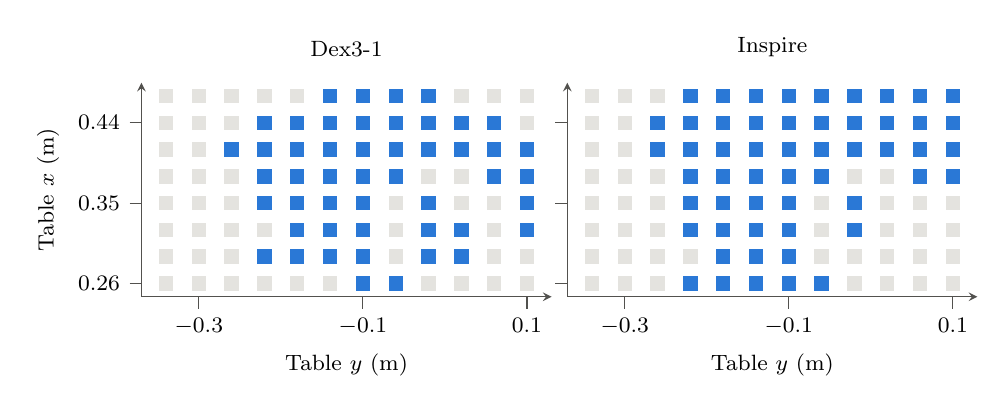
\begin{tikzpicture}
\begin{axis}[dexstyle, name=a, ylabel={Table $x$ (m)}, width=0.56\columnwidth, height=4.3cm, title={Dex3-1}, title style={font=\footnotesize}, ymajorgrids=false, xlabel={Table $y$ (m)}, xmin=-0.37, xmax=0.13, ymin=0.245, ymax=0.485, xtick={-0.3,-0.1,0.1}, ytick={0.26,0.35,0.44}]
\addplot[only marks,mark=square*,mark size=2.4pt,gridc] coordinates {(-0.34,0.26) (-0.30,0.26) (-0.26,0.26) (-0.22,0.26) (-0.18,0.26) (-0.14,0.26) (-0.02,0.26) (0.02,0.26) (0.06,0.26) (0.10,0.26) (-0.34,0.29) (-0.30,0.29) (-0.26,0.29) (-0.06,0.29) (0.06,0.29) (0.10,0.29) (-0.34,0.32) (-0.30,0.32) (-0.26,0.32) (-0.22,0.32) (-0.06,0.32) (0.06,0.32) (-0.34,0.35) (-0.30,0.35) (-0.26,0.35) (-0.06,0.35) (0.02,0.35) (0.06,0.35) (-0.34,0.38) (-0.30,0.38) (-0.26,0.38) (-0.02,0.38) (0.02,0.38) (-0.34,0.41) (-0.30,0.41) (-0.34,0.44) (-0.30,0.44) (-0.26,0.44) (0.10,0.44) (-0.34,0.47) (-0.30,0.47) (-0.26,0.47) (-0.22,0.47) (-0.18,0.47) (0.02,0.47) (0.06,0.47) (0.10,0.47)};
\addplot[only marks,mark=square*,mark size=2.4pt,dexblue] coordinates {(-0.10,0.26) (-0.06,0.26) (-0.22,0.29) (-0.18,0.29) (-0.14,0.29) (-0.10,0.29) (-0.02,0.29) (0.02,0.29) (-0.18,0.32) (-0.14,0.32) (-0.10,0.32) (-0.02,0.32) (0.02,0.32) (0.10,0.32) (-0.22,0.35) (-0.18,0.35) (-0.14,0.35) (-0.10,0.35) (-0.02,0.35) (0.10,0.35) (-0.22,0.38) (-0.18,0.38) (-0.14,0.38) (-0.10,0.38) (-0.06,0.38) (0.06,0.38) (0.10,0.38) (-0.26,0.41) (-0.22,0.41) (-0.18,0.41) (-0.14,0.41) (-0.10,0.41) (-0.06,0.41) (-0.02,0.41) (0.02,0.41) (0.06,0.41) (0.10,0.41) (-0.22,0.44) (-0.18,0.44) (-0.14,0.44) (-0.10,0.44) (-0.06,0.44) (-0.02,0.44) (0.02,0.44) (0.06,0.44) (-0.14,0.47) (-0.10,0.47) (-0.06,0.47) (-0.02,0.47)};
\end{axis}
\begin{axis}[dexstyle, at={(a.south east)}, xshift=0.2cm, anchor=south west, yticklabels={}, width=0.56\columnwidth, height=4.3cm, title={Inspire}, title style={font=\footnotesize}, ymajorgrids=false, xlabel={Table $y$ (m)}, xmin=-0.37, xmax=0.13, ymin=0.245, ymax=0.485, xtick={-0.3,-0.1,0.1}, ytick={0.26,0.35,0.44}]
\addplot[only marks,mark=square*,mark size=2.4pt,gridc] coordinates {(-0.34,0.26) (-0.30,0.26) (-0.26,0.26) (-0.02,0.26) (0.02,0.26) (0.06,0.26) (0.10,0.26) (-0.34,0.29) (-0.30,0.29) (-0.26,0.29) (-0.22,0.29) (-0.06,0.29) (-0.02,0.29) (0.02,0.29) (0.06,0.29) (0.10,0.29) (-0.34,0.32) (-0.30,0.32) (-0.26,0.32) (-0.06,0.32) (0.02,0.32) (0.06,0.32) (0.10,0.32) (-0.34,0.35) (-0.30,0.35) (-0.26,0.35) (-0.06,0.35) (0.02,0.35) (0.06,0.35) (0.10,0.35) (-0.34,0.38) (-0.30,0.38) (-0.26,0.38) (-0.02,0.38) (0.02,0.38) (-0.34,0.41) (-0.30,0.41) (-0.34,0.44) (-0.30,0.44) (-0.34,0.47) (-0.30,0.47) (-0.26,0.47)};
\addplot[only marks,mark=square*,mark size=2.4pt,dexblue] coordinates {(-0.22,0.26) (-0.18,0.26) (-0.14,0.26) (-0.10,0.26) (-0.06,0.26) (-0.18,0.29) (-0.14,0.29) (-0.10,0.29) (-0.22,0.32) (-0.18,0.32) (-0.14,0.32) (-0.10,0.32) (-0.02,0.32) (-0.22,0.35) (-0.18,0.35) (-0.14,0.35) (-0.10,0.35) (-0.02,0.35) (-0.22,0.38) (-0.18,0.38) (-0.14,0.38) (-0.10,0.38) (-0.06,0.38) (0.06,0.38) (0.10,0.38) (-0.26,0.41) (-0.22,0.41) (-0.18,0.41) (-0.14,0.41) (-0.10,0.41) (-0.06,0.41) (-0.02,0.41) (0.02,0.41) (0.06,0.41) (0.10,0.41) (-0.26,0.44) (-0.22,0.44) (-0.18,0.44) (-0.14,0.44) (-0.10,0.44) (-0.06,0.44) (-0.02,0.44) (0.02,0.44) (0.06,0.44) (0.10,0.44) (-0.22,0.47) (-0.18,0.47) (-0.14,0.47) (-0.10,0.47) (-0.06,0.47) (-0.02,0.47) (0.02,0.47) (0.06,0.47) (0.10,0.47)};
\end{axis}
\end{tikzpicture}
\caption{Measured grasp-and-lift workspace (scripted, per table position; filled = success). Dex3-1 49 of 96 cells,
Inspire 54 of 96. On the Inspire, failures at the robot's right edge (negative $y$) occur with small arm errors, so the
grasp fails there, not the arm's reach.}
\label{fig:reach}
\end{figure}

\begin{figure}[t]
\centering
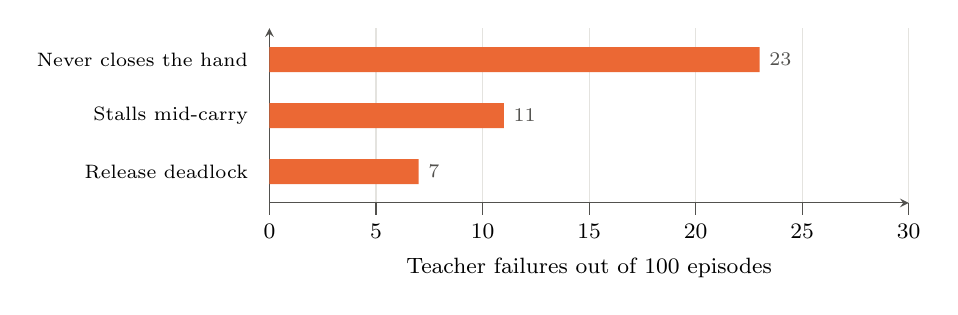
\begin{tikzpicture}
\begin{axis}[dexstyle, width=0.80\columnwidth, height=3.8cm, xbar, bar width=9pt, xmin=0, xmax=30, ymajorgrids=false, xmajorgrids, xlabel={Teacher failures out of 100 episodes},
  symbolic y coords={Release deadlock,Stalls mid-carry,Never closes the hand}, ytick=data, ytick style={draw=none}, enlarge y limits=0.28,
  nodes near coords, nodes near coords style={font=\scriptsize,text=ink}, y tick label style={font=\scriptsize}]
\addplot[fill=insorange,draw=none] coordinates {(7,Release deadlock) (11,Stalls mid-carry) (23,Never closes the hand)};
\end{axis}
\end{tikzpicture}
\caption{The Inspire teacher's 41 test failures, classified by re-running them. In 18 of the 23 ``never closes'' cases the
palm came within 1.5\,cm of the grasp pose.}
\label{fig:insfail}
\end{figure}

\textbf{Reading the failures.} Figure~\ref{fig:insfail} shows that most failures are decisions, not physical drops: only 2
of 41 ended early. The 0.7 threshold fixed the release deadlock on training layouts but likely blocks closing where grip
probability sits at 0.5--0.7. Both grip decisions are uncertain in this teacher, which one threshold cannot fix. The
held-out score of 85\% (13 clips) vs 59\% on 100 test layouts shows how much a small validation set can mislead; the test
layouts may also spread more widely across the workspace.

\textbf{Interpretation.} A task can remain identical while becoming substantially harder to execute because the robot's
embodiment is more complex. In our setting, the added dexterity brought no benefit for a cylindrical pick-and-place: the
working grip effectively squeezes with three fingers, and the hand tolerated less trajectory noise. We present this as an
observation, not a general law; Section~\ref{sec:limits} lists the confounds.

\section{Limitations}\label{sec:limits}
\begin{itemize}\setlength{\itemsep}{1pt}
\item \textbf{Simulation only.} No real-robot test; policies read true object state.
\item \textbf{One task, one training run per hand.} McNemar $p$-values cover layout variation, not training-seed
variation. Repeated seeds could shift these numbers.
\item \textbf{The hand comparison is confounded.} The hands differ in model quality (curated Menagerie vs corrected
URDF), grasp strategy, data, noise level, grip threshold and test layouts. A controlled comparison would disable two fingers on the same hand with everything else identical.
\item \textbf{Compute is estimated}, from per-model timings on a laptop CPU, not measured on robot hardware; it omits IK
and physics, which are identical across conditions.
\item \textbf{Assumed quantities.} Tube mass, rigid tube in the hand, and $S=0.3$ are assumptions.
\item \textbf{Scripted parts.} Approach and retreat paths and the grasp come from the robot side, so the demonstrations
do not determine every part of the motion.
\item \textbf{Post-hoc choices.} The ``released'' criterion change and the Inspire threshold are disclosed; the threshold
was chosen without validation or test layouts.
\item \textbf{Not done.} The planned generic-dataset ablation and an image-based teacher.
\end{itemize}

\section{Conclusion}
Calling a large policy only when it matters works, on one condition: the small policy must be trained for the states
it actually meets when deployed. On a simulated G1 picking up a tube, phase routing kept 76\% success (86\% for the
teacher alone) at an estimated 3 times less compute per step, while a random schedule with the same budget reached 43\%.
All of it was learned from demonstrations recorded with a phone. Next steps are a real-robot test, other tasks, an
image-based teacher, and a controlled comparison of hand complexity.

\section*{Code and Data Availability}
Code, trained models, processed episodes and per-episode results are in the project's public repository, submitted with
this paper; its README also links the raw recordings. Results can be reproduced without training
(\texttt{summarize\_results.py}, \texttt{eval\_policy.py}); on clean copies in a fresh environment, the first 10 test
layouts of all 4 conditions reproduced exactly on both hands (identical success and tick count, 40 of 40).

\section*{Acknowledgements}
AI assistance (Claude Code, Anthropic) was used for software development, analysis and drafting; the author directed the work and is responsible for its content.

\begin{thebibliography}{99}\small\setlength{\itemsep}{1pt}
\bibitem{act} T.~Z. Zhao, V.~Kumar, S.~Levine, C.~Finn. Learning fine-grained bimanual manipulation with low-cost hardware. \emph{RSS}, 2023.
\bibitem{dagger} S.~Ross, G.~Gordon, D.~Bagnell. A reduction of imitation learning and structured prediction to no-regret online learning. \emph{AISTATS}, 2011.
\bibitem{dart} M.~Laskey, J.~Lee, R.~Fox, A.~Dragan, K.~Goldberg. DART: Noise injection for robust imitation learning. \emph{CoRL}, 2017.
\bibitem{causalconfusion} P.~de~Haan, D.~Jayaraman, S.~Levine. Causal confusion in imitation learning. \emph{NeurIPS}, 2019.
\bibitem{copycat} C.~Wen, J.~Lin, T.~Darrell, D.~Jayaraman, Y.~Gao. Fighting copycat agents in behavioral cloning from observation histories. \emph{NeurIPS}, 2020.
\bibitem{distill} G.~Hinton, O.~Vinyals, J.~Dean. Distilling the knowledge in a neural network. \emph{NeurIPS Deep Learning Workshop}, 2015.
\bibitem{egomimic} S.~Kareer et al. EgoMimic: Scaling imitation learning via egocentric video. \emph{ICRA}, 2025.
\bibitem{dexcap} C.~Wang et al. DexCap: Scalable and portable mocap data collection system for dexterous manipulation. \emph{RSS}, 2024.
\bibitem{mujoco} E.~Todorov, T.~Erez, Y.~Tassa. MuJoCo: A physics engine for model-based control. \emph{IROS}, 2012.
\bibitem{menagerie} K.~Zakka et al. MuJoCo Menagerie: A collection of high-quality simulation models for MuJoCo. 2022. \url{https://github.com/google-deepmind/mujoco_menagerie}
\bibitem{unitreeros} Unitree Robotics. unitree\_ros. \url{https://github.com/unitreerobotics/unitree_ros}
\bibitem{zhang} Z.~Zhang. A flexible new technique for camera calibration. \emph{IEEE TPAMI}, 22(11), 2000.
\bibitem{apriltag} E.~Olson. AprilTag: A robust and flexible visual fiducial system. \emph{ICRA}, 2011.
\bibitem{apriltag2} J.~Wang, E.~Olson. AprilTag 2: Efficient and robust fiducial detection. \emph{IROS}, 2016.
\bibitem{ippe} T.~Collins, A.~Bartoli. Infinitesimal plane-based pose estimation. \emph{IJCV}, 109(3), 2014.
\bibitem{mcnemar} Q.~McNemar. Note on the sampling error of the difference between correlated proportions or percentages. \emph{Psychometrika}, 12(2), 1947.
\end{thebibliography}
\end{document}
